\documentclass{article}
% NeurIPS 2026 style; [preprint] shows author names. The footer is replaced below.
\usepackage[preprint]{neurips_2026}
\makeatletter
\renewcommand{\@noticestring}{ESE 5420 Final Project, University of Pennsylvania. Updated draft, November 2026.}
\makeatother

\usepackage[utf8]{inputenc}
\usepackage[T1]{fontenc}
\usepackage{hyperref}
\hypersetup{colorlinks=true,linkcolor=black,citecolor=black,urlcolor=blue}
\usepackage{url}
\usepackage{booktabs}
\usepackage{amsmath,amsfonts}
\usepackage{microtype}
\usepackage{xcolor}
\usepackage{graphicx}
\usepackage{enumitem}
\setlist{nosep}
\graphicspath{{figures/}}

\newcommand{\bp}{\,\mathrm{bp}}
\newcommand{\RMSE}{\operatorname{RMSE}}
% Tables are generated by src/render_final.py from results/*.json; edit captions here, not numbers.
\newcommand{\gentable}[2][\small]{{#1\setlength{\tabcolsep}{4pt}\input{generated/#2}}}

\title{Can Lagged Yield Changes Beat a Random Walk?\\
One-Day Forecasts of the 10-Year U.S.\ Treasury Yield}

\author{%
  Jonah Engelmann \qquad Leo Gordon \qquad Malcolm Siljehag Alencar \\
  \textmd{University of Pennsylvania, ESE 5420}
}

\begin{document}
\maketitle

\begin{abstract}
Can a model fitted to recent daily changes in the 10-year U.S.\ Treasury yield forecast the next day's change better than a random walk, which predicts no change? We separate two ways a model could help: more information (lagged changes of the 2- and 30-year yields, yield-curve spreads and recent volatility, alongside the 10-year yield's own lags) and more flexibility ($k$-nearest neighbors and random forests, alongside linear models). Every model is tuned on twelve expanding-window quarters of 2021--2023 and then scored once on 2024--2025, a period we had not examined. Before scoring, we committed to one primary comparison: the lasso on the rich inputs against the zero-change forecast. Its root mean squared error (RMSE) exceeds the zero-change forecast's by 0.003 basis points (bp), with a 95\% paired block-bootstrap interval of $[-0.017, 0.021]$\,bp: a tie. Refitted on 2020--2023, the tuned lasso keeps none of its 18 inputs. None of the seven secondary models beats the random walk either; every interval contains zero. The primary interval bounds the improvement from the rich inputs at 0.017\,bp, or 0.3\% of the random walk's RMSE. Our earlier test on 2023, rerun with a corrected $k$NN, gives the same answer.
\end{abstract}

\section{Introduction}
Daily changes in long-term interest rates matter to anyone who holds or hedges bonds: a change of a few basis points in the 10-year Treasury yield moves the value of large portfolios, and the 10-year yield is a reference rate for mortgages and corporate borrowing. A forecast of tomorrow's change is only useful, however, if it beats the simplest possible forecast: that tomorrow's yield equals today's. This \emph{random walk} benchmark is famously hard to beat out of sample. \citet{meese1983} found that structural models did not beat it for exchange rates, and \citet{duffee2002} and \citet{diebold2006} report that it is a demanding benchmark for Treasury yields at short horizons.

We ask a narrow, testable version of the question: \emph{do recent daily yield changes predict the next change of the 10-year yield better than a forecast of zero change, by more than the sampling error of the comparison?} A finding that they do would point to short-term momentum or mean reversion. A careful null result is also informative, because its confidence interval bounds how much predictive information this kind of model can extract.

Our early draft answered this for one model and one test year: ordinary least squares (OLS) on lagged 10-year changes tied the random walk in 2023. A tie could have two causes: the model may see too little information, or it may be too rigid to use what it sees. We separate the two causes with a two-by-two design: \{10-year lags only, rich cross-maturity inputs\} $\times$ \{linear, flexible\}. We tune every model on data up to 2023 and score each one once on 2024--2025. Because eight models are compared, we wrote down one primary comparison before scoring and treat the other seven as secondary. Our contributions are:
\begin{itemize}[leftmargin=*]
  \item a time-ordered comparison of eight forecasts that separates information from flexibility, with every learned step, including feature scaling, fitted inside each training window;
  \item a pre-registered test on a fresh period, scored once, with paired block-bootstrap intervals that respect serial dependence and a correction for the secondary comparisons;
  \item a clear answer with a bound: every model ties the random walk, and the primary model is at most 0.017\,bp (0.3\%) better than zero change; tuned models collapse towards a constant forecast;
  \item a reproducibility fix: daily changes are whole basis points, so $k$NN faces many exactly tied neighbors, and library tie-breaking changed our results; we give an order-independent version.
\end{itemize}

\section{Related work}\label{sec:related}
\paragraph{The random walk benchmark.} \citet{meese1983} showed that exchange-rate models fitted in sample did not beat a random walk out of sample. For the term structure, \citet{duffee2002} found that completely affine models forecast Treasury yields worse than a random walk, and the dynamic Nelson--Siegel model of \citet{diebold2006} beats it mainly at horizons of six and twelve months rather than at one month. We study a much shorter horizon, one trading day, where the random walk should be hardest to beat.

\paragraph{Out-of-sample predictability.} \citet{welch2008} showed that variables that predict equity returns in sample mostly fail out of sample, and \citet{campbell2008} argued that even a small out-of-sample $R^2$ can be economically meaningful. Machine learning has improved forecasts of monthly stock returns \citep{gu2020} and of bond excess returns over one year \citep{bianchi2021}, but these studies forecast at monthly or longer horizons with large panels of predictors. We ask whether a small set of lagged yield variables, with linear or flexible models, carries any next-day information.

\paragraph{Evaluation.} Shuffled $K$-fold cross-validation lets a model train on days after the days it predicts; expanding-window validation keeps time order \citep{bergmeir2012}. To compare forecasts on serially dependent data we use a paired moving-block bootstrap \citep{kunsch1989} in its circular form \citep{politis1992}, close in spirit to tests of equal predictive accuracy \citep{diebold1995}. Comparing many models on one test set invites data snooping \citep{white2000}, which is why we name one primary comparison in advance.

\section{Data}\label{sec:data}
\paragraph{Source and size.} We use the U.S.\ Department of the Treasury's Daily Treasury Par Yield Curve Rates: the archive file for 2020--2023 and the files for 2024 and 2025 \citep{treasury2020,treasury2024}. These are public U.S.\ government data. Together they hold 1,500 trading days from 2 January 2020 to 31 December 2025, with par yields at 13 or 14 maturities (a 1.5-month maturity appears in 2025; we do not use it). There are no duplicate dates, and the 2-, 10- and 30-year yields, the only ones we use, have no missing values. We sort by date and difference consecutive trading days without filling non-trading days. Table~\ref{tab:data} gives the size and volatility of each year.

\begin{table}[t]
  \caption{Observations by year and the RMSE of the zero-change forecast, which equals the root mean square of the daily change and measures how volatile each year was. The first change of 2020 has no predecessor; later years difference against the previous year's last quote. The last two columns give each year's role in the two studies of Section~\ref{sec:setup}.}
  \label{tab:data}
  \centering
  \gentable{tab_data}
\end{table}

\paragraph{Target and inputs.} Let $r^{(m)}_t$ be the $m$-year par yield on trading day $t$, in percent. The target is the next daily change of the 10-year yield in basis points, and the simplest inputs are its last $p$ changes:
\begin{equation}
  y_t = 100\,\big(r^{(10)}_t - r^{(10)}_{t-1}\big) \bp, \qquad x_t^{(p)} = (y_{t-1}, \ldots, y_{t-p})^\top \in \mathbb{R}^p .
  \label{eq:features}
\end{equation}
The \emph{rich} inputs add the last $p$ daily changes of the 2- and 30-year yields, the previous day's 2s10s and 10s30s spreads, $100(r^{(10)}_{t-1} - r^{(2)}_{t-1})$ and $100(r^{(30)}_{t-1} - r^{(10)}_{t-1})$, and the sample standard deviation of the 10-year change over days $t-20, \ldots, t-1$, for $3p+3$ inputs in all. Every input is known before $r^{(10)}_t$ is published. Yields are quoted to two decimals, so every change is a whole number of basis points; across the six years $y_t$ takes only 46 distinct values.

\paragraph{Why the data start in 2020.} Treasury's archive goes back to 1990, but our training data start on 2 January 2020, for two reasons. First, the 2023 study (Section~\ref{sec:setup}) was designed and run on the 2020--2023 file, and its result stays in the paper as reported; starting the final study on the same date keeps the two studies comparable. Second, before opening the test period we checked, on validation data only, whether the start date matters. We compared training from 2020 with training from 2021, which drops the year of the COVID-19 shock, on the same eight quarters, 2022\,Q1 to 2023\,Q4. No model's best validation RMSE changed by more than 0.018\,bp (Appendix~\ref{app:start}), far less than the quarter-to-quarter variation. Longer histories would give the flexible models several times more data; we did not test them, and list them as the most direct extension in Section~\ref{sec:discussion}.

\section{Methods}\label{sec:methods}
\paragraph{References.} The \emph{zero-change forecast}, $\widehat y_t = 0$ or equivalently $\widehat r^{(10)}_t = r^{(10)}_{t-1}$, is a random walk in the yield level and has no parameters; it is the benchmark every model must beat. The \emph{training mean}, $\widehat y_t = \bar y_{\text{train}}$, forecasts the average daily change of the training window. It is the forecast that any model reduces to when it ignores its inputs, so it separates the value of the inputs from the value of an estimated drift.

\paragraph{Linear models.} \emph{OLS} on 10-year lags, $\widehat y_t = \widehat\beta_0 + \widehat\beta^\top x_t^{(p)}$, is an AR($p$) model for the daily changes, that is, an ARIMA($p$,1,0) model for the yield with drift, fitted by least squares; the zero-change forecast is ARIMA(0,1,0) without drift. On the rich inputs we fit \emph{ridge} regression \citep{hoerl1970} and the \emph{lasso} \citep{tibshirani1996}, which shrink the coefficients towards zero; the lasso can set them exactly to zero and so select inputs. Their inputs are standardized with the training window's means and standard deviations.

\paragraph{Flexible models.} \emph{$k$-nearest neighbors} predicts the mean target of the $k$ training days whose inputs are closest in Euclidean distance, after standardizing each input with the training window's standard deviation. Because daily changes are whole basis points, many training days often lie at exactly the $k$-th smallest distance $d_{(k)}$ from a query, and library implementations then choose among them by row order or search-tree layout. On our data, three scikit-learn search algorithms gave single 2023 forecasts that differed by up to 6\,bp for $k=3$. We remove the arbitrariness: with $\mathcal N_{<}$ the days strictly closer than $d_{(k)}$ and $\mathcal T$ the days tied at $d_{(k)}$,
\begin{equation}
  \widehat y_t = \frac1k \Big( \sum_{i \in \mathcal N_{<}} y_i + \frac{k - |\mathcal N_{<}|}{|\mathcal T|} \sum_{i \in \mathcal T} y_i \Big),
  \label{eq:knn}
\end{equation}
which equals the average prediction over all ways of breaking the ties. It matches scikit-learn to machine precision when there are no ties and gives identical forecasts under any reordering of the training days. A \emph{random forest} \citep{breiman2001} averages regression trees fitted to bootstrap samples, each split choosing among a random subset of inputs. To avoid reporting the best of several random runs, every forest is the average of five forests of 100 trees with seeds 0--4, fixed in advance; we also report the spread across the five.

\section{Experimental setup}\label{sec:setup}
\paragraph{Two studies.} The \emph{2023 study} is the experiment of our early draft, kept as it was designed: OLS ($p \in \{1, \ldots, 5\}$) and $k$NN ($p \in \{1,\dots,5\}$, $k \in \{3, 5, 10, 20, 40\}$) are tuned on the eight quarters of 2021--2022, refitted on 2020--2022, and scored on 2023. We rerun it with the corrected $k$NN and add the training mean, but change nothing else. Because 2023 has now been inspected, every new model and feature moves to the \emph{final study}: all eight forecasts of Section~\ref{sec:methods} are tuned on the twelve quarters 2021\,Q1 to 2023\,Q4, refitted once on 2020--2023, and scored once on the 499 daily changes of 2024--2025.

\paragraph{Tuning.} Each validation quarter is predicted by a model fitted on every earlier day from January 2020 (an expanding window), so no fold ever trains on the future. Every candidate is scored on the same validation days. For each model we select the candidate with the lowest mean of the quarterly RMSEs, breaking ties towards fewer lags and then the simpler setting (a larger penalty, a larger leaf, a smaller $k$). The final study searches $p \in \{1, \ldots, 5\}$ for every model except the training mean; $k \in \{3, 5, 10, 20, 40, 80, 160, 320\}$, capped at the number of training days; ridge penalties $\alpha \in \{10^0, 10^{0.5}, \ldots, 10^5\}$; lasso penalties $\alpha \in \{10^{-3}, 10^{-2.75}, \ldots, 10^{0.5}\}$; and random forests with a minimum leaf size in $\{10, 40, 160\}$ and either all inputs or $\lfloor\sqrt{n}\rfloor$ of the $n$ inputs at each split (273 candidates in all; Appendix~\ref{app:grids}). When forecasting the test period, the refitted model uses the observed earlier days as lags but is never refitted on them.

\paragraph{Pre-registration.} Before scoring 2024--2025 we committed a pre-registration to the project repository (commit \texttt{9f6d56a}, 27 November 2026), and the scoring script refuses to run without it. It fixes the primary comparison, the \emph{lasso on the rich inputs against the zero-change forecast, pooled over 2024--2025}, and the reading of its interval: the lasso beats the random walk if the whole interval lies below zero, loses if it lies above, and ties otherwise. It also lists the secondary comparisons, the grids, the selection rule and the settings selected on validation, all fixed before the test was scored.

\paragraph{Metric.} For model $m$ evaluated on $n$ days,
\begin{equation}
  \RMSE_m = \Big(\tfrac{1}{n}\textstyle\sum_{t=1}^{n} (y_t - \widehat y_{m,t})^2\Big)^{1/2}, \qquad D_m = \RMSE_m - \RMSE_0,
  \label{eq:delta}
\end{equation}
in basis points, where $\RMSE_0$ is the zero-change forecast's. A negative $D_m$ means the model beats the random walk.

\paragraph{Error bars.} For validation we report the mean $\pm$ the sample standard deviation of the quarterly RMSEs, which shows how the error level moves between quarters, and the paired per-quarter differences $D_{m,q} = \RMSE_{m,q} - \RMSE_{0,q}$, which measure the model difference directly. On the test period, daily changes are serially dependent and their volatility clusters, so an i.i.d.\ bootstrap would understate uncertainty. We use a paired circular moving-block bootstrap: draw blocks of 20 consecutive test days (about one trading month) with replacement, letting a block that runs past the end wrap around to the start, until $n$ days are drawn; recompute $D_m$ on the \emph{same} resampled days; repeat 10,000 times (seed 5420); and report the 2.5\% and 97.5\% percentiles. Every model is resampled on the same days. We compute intervals for 2024, 2025 and the pooled period, and repeat the pooled bootstrap with 10- and 30-day blocks (5,000 resamples each). The intervals are conditional on the fitted models and do not include uncertainty from hyperparameter selection.

\paragraph{Multiple comparisons.} Beside the primary comparison there are seven secondary ones: every other model against zero change, pooled. With seven 95\% intervals, one could exclude zero by chance alone, so for each we also report a Bonferroni interval at level $1 - 0.05/7 \approx 99.3\%$, which controls the chance of any false finding among the seven at 5\%.

\paragraph{Reproducibility.} The analysis is deterministic: the folds, the tie-aware $k$NN and the forest seeds are fixed, and two complete runs give byte-identical results. Three scripts produce every number, table and figure in this paper from the raw Treasury files: one for the 2023 study, one for the final study, and one for the tables and figures. Code and data: \url{https://github.com/lourinhos/treasuries}. We used Python 3.15, NumPy 2.5, pandas 3.1, scikit-learn 1.9 and Matplotlib 3.11.

\section{Results}\label{sec:results}
\subsection{The 2023 study, rerun}
Table~\ref{tab:cv2023} gives the validation results and Table~\ref{tab:test2023} the single 2023 evaluation. The OLS results are unchanged from the early draft: the selected model, $\widehat y_t = 0.269 + 0.033\,y_{t-1}$\,bp, is close to the training mean of 0.278\,bp per day, and it ties the zero-change forecast ($D = +0.025$\,bp, interval $[-0.018, 0.066]$). The interval bounds what lagged 10-year changes delivered in 2023: OLS was at most 0.018\,bp better than zero change, 0.24\% of the random walk's RMSE. With the corrected $k$NN, the selected configuration is the same as before ($p=2$, $k=40$) and its difference moves from $+0.112$ to $+0.106$\,bp, with interval $[0.013, 0.194]$\,bp: $k$NN was significantly \emph{worse} than the random walk in 2023, and stays so with 10- and 30-day blocks ($[0.009, 0.199]$ and $[0.009, 0.197]$). The training mean ties ($+0.005$, $[-0.030, 0.040]$). In validation, no forecast beats zero change on average, and each selected forecast wins only three of the eight quarters.

\begin{table}[t]
  \caption{2023 study: validation RMSE over the eight quarters of 2021--2022 (mean $\pm$ sample s.d.\ across quarters), and the paired per-quarter difference $D$ from zero change (mean $\pm$ s.d.; negative favors the model) with the number of quarters in which the model beats zero change. The lowest mean RMSE selects each model's setting.}
  \label{tab:cv2023}
  \centering
  \gentable{tab_cv2023}
\end{table}

\begin{table}[t]
  \caption{2023 study: held-out 2023 forecasts ($n=250$ days). $D$ is the model's RMSE minus the zero-change RMSE. Intervals: paired circular block bootstrap, 20-day blocks, 10,000 resamples. Only $k$NN's interval excludes zero, and it lies above zero: $k$NN is worse than the random walk.}
  \label{tab:test2023}
  \centering
  \gentable{tab_test2023}
\end{table}

\subsection{Final study: validation}
Table~\ref{tab:cvfinal} summarizes the selected setting of each model over the twelve validation quarters. No model beats the zero-change forecast on average: the paired differences range from $+0.001$\,bp (ridge) to $+0.022$\,bp (OLS), each model wins between four and seven of the twelve quarters, and every difference is a small fraction of its own quarter-to-quarter spread. Figure~\ref{fig:validation} shows why. The error level more than doubles between 2021\,Q2 (3.48\,bp) and 2023\,Q1 (8.38\,bp) as rate volatility rises, while the eight models stay within about 0.1\,bp of the zero-change forecast in every quarter.

Validation also pushed every model towards a constant forecast. Both $k$NN models selected $k=320$, the largest value in the widened grid; $k$NN improves only as it approaches the training mean, which answers the question that motivated the wider grid. Both random forests selected the largest leaf size, ridge a heavy penalty ($\alpha = 10^4$), and the lasso the second-largest penalty in its grid.

\begin{table}[t]
  \caption{Final study: validation over the twelve quarters 2021\,Q1--2023\,Q4, training from 2020. For each model, the setting with the lowest mean quarterly RMSE among its candidates (Cand.), its RMSE (mean $\pm$ s.d.), its paired per-quarter difference $D$ from zero change (mean $\pm$ s.d.), and the quarters in which it beats zero change. No model beats zero change on average.}
  \label{tab:cvfinal}
  \centering
  \gentable[\footnotesize]{tab_cvfinal}
\end{table}

\begin{figure}[t]
  \centering
  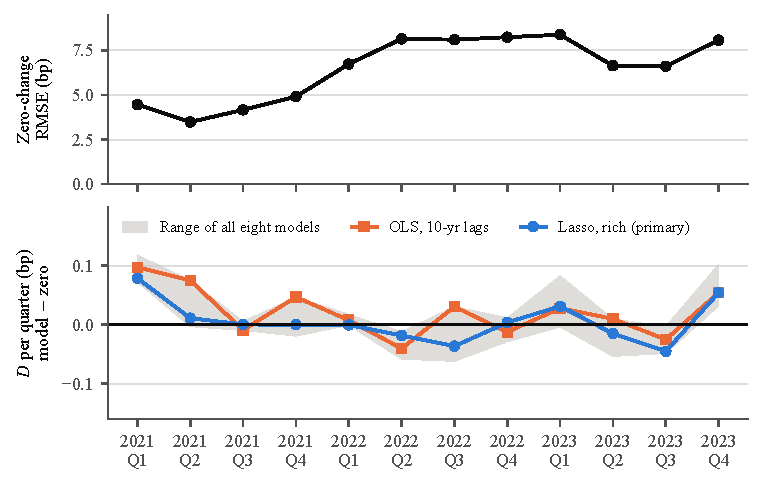
\includegraphics[width=\linewidth]{validation_quarters.pdf}
  \caption{Final study, validation by quarter. Top: RMSE of the zero-change forecast, which tracks rate volatility. Bottom: the paired difference $D$ between each selected model and zero change in the same quarter; the band spans all eight models. The error level changes by about 5\,bp across quarters; the models differ from the random walk by about 0.1\,bp at most.}
  \label{fig:validation}
\end{figure}

\subsection{Final study: the 2024--2025 test}
\paragraph{Primary comparison.} The lasso on the rich inputs has a pooled RMSE of 5.341\,bp against 5.338\,bp for the zero-change forecast: $D = +0.003$\,bp with 95\% interval $[-0.017, 0.021]$\,bp (Table~\ref{tab:testfinal}). The interval contains zero, so by the pre-registered rule the lasso \emph{ties} the random walk. The result does not depend on the block length ($[-0.017, 0.022]$ with 10-day blocks, $[-0.017, 0.021]$ with 30-day blocks). The reason is visible in the fitted model: refitted on 2020--2023 at the selected penalty, the lasso sets all 18 coefficients to zero, so its forecast is the constant 0.242\,bp per day, the mean change of its training days. Validation chose a penalty at which, on the full training data, the lasso ignores every input. The interval also bounds what the rich inputs could have delivered: at most 0.017\,bp, 0.3\% of the random walk's RMSE.

\begin{table}[t]
  \caption{Final study: the 2024--2025 test ($n = 499$ days; 250 in 2024, 249 in 2025), scored once. RMSE and $D$ in bp; $D$ is the model's RMSE minus the zero-change RMSE (negative favors the model). Intervals: paired circular block bootstrap, 20-day blocks, 10,000 resamples. The lasso is the pre-registered primary comparison; the Bonferroni intervals (level $1-0.05/7$) correct the seven secondary comparisons. Every interval contains zero.}
  \label{tab:testfinal}
  \centering
  \gentable[\footnotesize]{tab_testfinal}
\end{table}

\paragraph{Secondary comparisons.} No model's 95\% interval excludes zero (Table~\ref{tab:testfinal} and Figure~\ref{fig:key}), so no Bonferroni interval does either. The linear models are all near-constant forecasts. Refitted on 2020--2023, OLS is $\widehat y_t = 0.208 - 0.0003\,y_{t-1}$, practically the training mean of 0.208\,bp; the heavily penalized ridge forecast is within 0.001\,bp of the training mean in RMSE. OLS, ridge and the training mean all tie the random walk with $D = +0.002$\,bp. The flexible models on 10-year lags come closest to an improvement: the random forest has $D = -0.013$\,bp, $[-0.036, 0.011]$, and all five seeds agree on the sign ($-0.011$ to $-0.014$\,bp); $k$NN has $D = -0.009$\,bp, $[-0.034, 0.016]$. Neither interval excludes zero even at 95\%, so we do not read them as evidence of an improvement. On the rich inputs, the flexible models are no better: $k$NN $+0.009$\,bp and the random forest $0.000$\,bp. More information did not help any model class, and more flexibility helped, if at all, by less than the sampling error.

\paragraph{By year.} The per-year results follow the drift of each year. Over 2020--2023 the 10-year yield rose on average, so the near-constant linear models and the training mean forecast a rise of about 0.2\,bp per day. The yield did rise on average in 2024 (by 0.28\,bp per day) and fell in 2025 (by 0.16\,bp per day), so these models are slightly better than zero change in 2024 ($D \approx -0.006$\,bp) and slightly worse in 2025 ($D \approx +0.011$ to $+0.014$\,bp). No per-year interval excludes zero (Figure~\ref{fig:key}).

\begin{figure}[t]
  \centering
  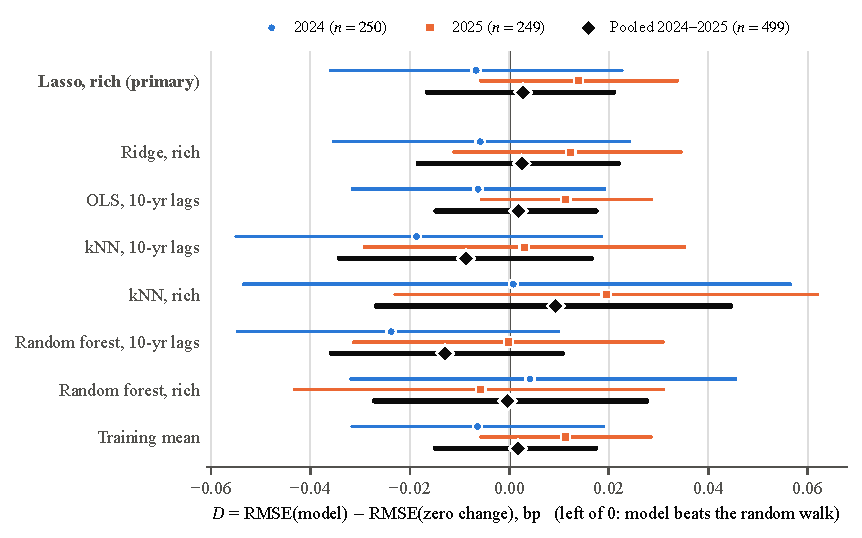
\includegraphics[width=\linewidth]{test_differences.pdf}
  \caption{The key result: each model's RMSE minus the zero-change RMSE on the 2024--2025 test, with 95\% paired block-bootstrap intervals for 2024, 2025 and both years pooled. A model beats the random walk only if its interval lies entirely left of zero. All intervals contain zero, including the pre-registered primary comparison (top).}
  \label{fig:key}
\end{figure}

\section{Discussion and limitations}\label{sec:discussion}
\paragraph{What the tie means.} In two separate test periods, no forecast built from recent yield changes predicted the next day's change of the 10-year yield better than no change. The tie is tight: the primary interval rules out an improvement larger than 0.017\,bp, against a typical daily move of about 5\,bp. The pattern in validation explains the result: with more data or more freedom, every model moved towards a constant, and the best constant, the historical drift, is itself no better than zero. This is what an efficient market would produce at a one-day horizon: public information in yesterday's yield curve is already in today's price.

\paragraph{Volatility, not direction, drives the error.} The error of every forecast rose and fell with rate volatility, which varied far more across quarters than any difference between models. A volatility model such as ARCH \citep{engle1982} or GARCH \citep{bollerslev1986} could forecast how large tomorrow's change will be, and so how large the random walk's error will be, but not its sign, which is what a better point forecast requires. Forecasting volatility is a different question from ours, and probably a more answerable one.

\paragraph{Limitations.}
\begin{itemize}[leftmargin=*]
  \item \emph{One target and one horizon.} We forecast only the 10-year yield, one trading day ahead, from end-of-day quotes. Other maturities, intraday data or multi-day horizons could behave differently.
  \item \emph{A narrow information set.} All inputs come from the Treasury yield curve itself. We used no macroeconomic releases, policy announcements, futures, or news, which drive many large daily moves.
  \item \emph{Short history.} Training starts in 2020 (Section~\ref{sec:data}). The flexible models in particular might do better with the archive back to 1990, though that history spans very different rate regimes.
  \item \emph{Two test years.} The test covers 2024 and 2025 only. The per-year results already differ in sign for the drift-based forecasts, so other periods could give somewhat different differences, although a 95\% interval that excludes zero would need an effect about twice as large as the largest we saw.
  \item \emph{Conditional intervals.} The bootstrap treats the fitted models as fixed and ignores uncertainty from tuning. The Bonferroni correction is conservative, but with every 95\% interval already containing zero, it changes no conclusion.
  \item \emph{Scope of models.} We did not fit moving-average terms (OLS covers ARIMA($p$,1,0) only) or models of a time-varying conditional mean. We also refit each model once rather than re-estimating it during the test period; with near-constant forecasts we expect this to matter little.
  \item \emph{RMSE only.} We measure accuracy, not economic value; a forecast that ties in RMSE could still differ in, for example, the direction it gets right on large-move days.
\end{itemize}

\section{Conclusion}
No. Over 2024--2025, a fresh test period scored once, neither more information (cross-maturity changes, spreads and recent volatility) nor more flexibility ($k$-nearest neighbors, random forests) produced a forecast of the next day's 10-year Treasury yield change that beats the random walk. The pre-registered primary comparison, the lasso on the rich inputs, ties zero change ($+0.003$\,bp, $[-0.017, 0.021]$) and in fact uses none of its inputs; every other model ties as well. Lagged yield information is therefore worth at most a few hundredths of a basis point of RMSE at this horizon, and the error of every forecast is governed by volatility, not by the choice of model.

\begin{ack}
% TODO (group): check that this statement matches how each of us used AI tools during the project, and edit it if not.
We thank the course staff for their feedback on the early draft. We used Claude (Anthropic), through Claude Code, to reorganize the code repository, implement the tie-aware $k$NN and the final experiment, table and figure scripts, and draft and edit the text of this paper from our experiment plan and the feedback. The research question, the study design, the choice of primary comparison and of the training start, and the interpretation are ours, and we are responsible for all code and text.
\end{ack}

{\raggedright
\begin{thebibliography}{99}
\bibitem[Bergmeir and Ben\'itez(2012)]{bergmeir2012}
C.~Bergmeir and J.~M. Ben\'itez. On the use of cross-validation for time series predictor evaluation. \emph{Information Sciences}, 191:192--213, 2012.

\bibitem[Bianchi et~al.(2021)Bianchi, B\"uchner, and Tamoni]{bianchi2021}
D.~Bianchi, M.~B\"uchner, and A.~Tamoni. Bond risk premiums with machine learning. \emph{The Review of Financial Studies}, 34(2):1046--1089, 2021.

\bibitem[Bollerslev(1986)]{bollerslev1986}
T.~Bollerslev. Generalized autoregressive conditional heteroskedasticity. \emph{Journal of Econometrics}, 31(3):307--327, 1986.

\bibitem[Breiman(2001)]{breiman2001}
L.~Breiman. Random forests. \emph{Machine Learning}, 45(1):5--32, 2001.

\bibitem[Campbell and Thompson(2008)]{campbell2008}
J.~Y. Campbell and S.~B. Thompson. Predicting excess stock returns out of sample: Can anything beat the historical average? \emph{The Review of Financial Studies}, 21(4):1509--1531, 2008.

\bibitem[Diebold and Li(2006)]{diebold2006}
F.~X. Diebold and C.~Li. Forecasting the term structure of government bond yields. \emph{Journal of Econometrics}, 130(2):337--364, 2006.

\bibitem[Diebold and Mariano(1995)]{diebold1995}
F.~X. Diebold and R.~S. Mariano. Comparing predictive accuracy. \emph{Journal of Business \& Economic Statistics}, 13(3):253--263, 1995.

\bibitem[Duffee(2002)]{duffee2002}
G.~R. Duffee. Term premia and interest rate forecasts in affine models. \emph{The Journal of Finance}, 57(1):405--443, 2002.

\bibitem[Engle(1982)]{engle1982}
R.~F. Engle. Autoregressive conditional heteroscedasticity with estimates of the variance of United Kingdom inflation. \emph{Econometrica}, 50(4):987--1007, 1982.

\bibitem[Gu et~al.(2020)Gu, Kelly, and Xiu]{gu2020}
S.~Gu, B.~Kelly, and D.~Xiu. Empirical asset pricing via machine learning. \emph{The Review of Financial Studies}, 33(5):2223--2273, 2020.

\bibitem[Hoerl and Kennard(1970)]{hoerl1970}
A.~E. Hoerl and R.~W. Kennard. Ridge regression: Biased estimation for nonorthogonal problems. \emph{Technometrics}, 12(1):55--67, 1970.

\bibitem[K\"unsch(1989)]{kunsch1989}
H.~R. K\"unsch. The jackknife and the bootstrap for general stationary observations. \emph{The Annals of Statistics}, 17(3):1217--1241, 1989.

\bibitem[Meese and Rogoff(1983)]{meese1983}
R.~A. Meese and K.~Rogoff. Empirical exchange rate models of the seventies: Do they fit out of sample? \emph{Journal of International Economics}, 14(1--2):3--24, 1983.

\bibitem[Politis and Romano(1992)]{politis1992}
D.~N. Politis and J.~P. Romano. A circular block-resampling procedure for stationary data. In R.~LePage and L.~Billard, editors, \emph{Exploring the Limits of Bootstrap}, pages 263--270. Wiley, 1992.

\bibitem[Tibshirani(1996)]{tibshirani1996}
R.~Tibshirani. Regression shrinkage and selection via the lasso. \emph{Journal of the Royal Statistical Society: Series B}, 58(1):267--288, 1996.

\bibitem[{U.S. Department of the Treasury}(2026a)]{treasury2020}
U.S.\ Department of the Treasury. Daily Treasury par yield curve rates, 2020--2023 (archive file). \url{https://home.treasury.gov/resource-center/data-chart-center/interest-rates/daily-treasury-rate-archives/par-yield-curve-rates-2020-2023.csv}. Accessed November 2026.

\bibitem[{U.S. Department of the Treasury}(2026b)]{treasury2024}
U.S.\ Department of the Treasury. Daily Treasury par yield curve rates, 2024 and 2025. \url{https://home.treasury.gov/resource-center/data-chart-center/interest-rates/TextView?type=daily_treasury_yield_curve}. Accessed November 2026.

\bibitem[Welch and Goyal(2008)]{welch2008}
I.~Welch and A.~Goyal. A comprehensive look at the empirical performance of equity premium prediction. \emph{The Review of Financial Studies}, 21(4):1455--1508, 2008.

\bibitem[White(2000)]{white2000}
H.~White. A reality check for data snooping. \emph{Econometrica}, 68(5):1097--1126, 2000.
\end{thebibliography}
}

\appendix
\section{Search grids}\label{app:grids}
Every model except the references searches the lag length $p \in \{1, \ldots, 5\}$; the rich inputs then have $3p+3$ columns. The other settings are: $k$NN, $k \in \{3, 5, 10, 20, 40, 80, 160, 320\}$, capped at the number of training days (which only affects $k=320$ in the earliest folds); ridge, $\alpha \in \{10^{0}, 10^{0.5}, \ldots, 10^{5}\}$ (11 values); lasso, $\alpha \in \{10^{-3}, 10^{-2.75}, \ldots, 10^{0.5}\}$ (15 values); random forest, minimum leaf size $\{10, 40, 160\}$ and inputs tried per split $\{$all, $\lfloor\sqrt n\rfloor\}$, dropping the second where it equals the first. Ridge and the lasso follow scikit-learn's scaling of the penalty: ridge minimizes $\|y - \beta_0 - X\beta\|^2 + \alpha\|\beta\|_2^2$ and the lasso $\frac{1}{2n}\|y - \beta_0 - X\beta\|^2 + \alpha\|\beta\|_1$, both on standardized inputs. The validation RMSE of every candidate is in \texttt{results/final\_2020.json} in the repository.

\section{Training from 2020 or from 2021}\label{app:start}
Table~\ref{tab:start} compares the two training starts on the eight validation quarters they share. Each model's setting is selected separately for each start, using these eight quarters only. The difference between starts is at most 0.018\,bp for every model. Selected on these eight quarters alone, all eight models look slightly better than zero change under the 2020 start and seven of eight under the 2021 start (down to $-0.030$\,bp). Part of this is the rising drift of 2022, which the training mean captures; part is selection, since with up to 75 candidates per model the best of many is expected to look slightly lucky. Selected over all twelve quarters, the same models show no advantage (Table~\ref{tab:cvfinal}), and none shows one on the test period.

\begin{table}[h]
  \caption{Mean validation RMSE (bp) over 2022\,Q1--2023\,Q4 for each model's best setting, training from 2020 or from 2021 (which drops the year of the COVID-19 shock), the difference (2021 minus 2020), and the paired difference $D$ from zero change under each start. No test data were used.}
  \label{tab:start}
  \centering
  \gentable{tab_trainstart}
\end{table}

\end{document}
